\documentclass[11pt]{article}
\usepackage[margin=1in]{geometry}
\usepackage{amsmath,amssymb,amsthm,mathtools}
\usepackage{booktabs,tabularx,array}
\usepackage{graphicx}
\usepackage{xcolor}
\usepackage{enumitem}
\usepackage[hidelinks]{hyperref}

\graphicspath{{../figures/}{figures/}}
% Placeholder for numbers that come from running src/load_data.py on the real data
\newcommand{\fillin}[1]{\textcolor{red}{\textbf{[#1]}}}
% Include a figure if it exists, otherwise draw a placeholder box (keeps Overleaf compiling)
\newcommand{\maybefig}[2]{%
  \IfFileExists{../figures/#1}{\includegraphics[width=#2]{#1}}{%
  \IfFileExists{figures/#1}{\includegraphics[width=#2]{#1}}{%
  \fbox{\parbox[c][4cm][c]{#2}{\centering\small Run \texttt{python src/load\_data.py}\\
  to create \texttt{figures/\detokenize{#1}}}}}}}
\newcommand{\owner}[2]{\par\noindent\textit{Owner: #1 \hfill Checked by: #2}\par\medskip}

\theoremstyle{plain}
\newtheorem{theorem}{Theorem}
\newtheorem{proposition}[theorem]{Proposition}
\theoremstyle{definition}
\newtheorem{definition}{Definition}
\newtheorem{assumption}{Assumption}

\newcommand{\R}{\mathbb{R}}
\newcommand{\N}{\mathbb{N}}
\newcommand{\V}{\mathcal{V}}
\newcommand{\Vs}{|\mathcal{V}|}
\newcommand{\bx}{\mathbf{x}}
\newcommand{\bw}{\mathbf{w}}
\DeclareMathOperator*{\argmax}{arg\,max}

\title{DS5020 Final Project -- Iteration 2\\[2pt]
\large Naive Bayes Spam Classification: Definitions, Derivations, Data and Simulation}
\author{Jeevan Mandala \and Anand Joel Battula}
\date{Fall 2026}

\begin{document}
\maketitle

\noindent\textbf{Project Leader (Iteration 2):} Jeevan Mandala\\
\textbf{Repository:} 
\href{https://github.com/Jeev2727/Ds5020-naive-bayes-classifier}{\texttt{Github repo}} \\
\textbf{Overleaf:} \href{https://www.overleaf.com/project/6af8e7c4a2e68e546f457ae0/share#96183df2ea7e80e3119e925675021469490224631bf61309}{\texttt{Latex code}} 

\tableofcontents

%======================================================================
\section{Team and Task Ownership}
Each derivation and math question has one owner and one checker. The owner writes and signs
the result; the checker re-derives it independently and signs ``checked by''. Either member can
explain any part at the check-in.

\begin{center}
\begin{tabularx}{\textwidth}{@{}llXll@{}}
\toprule
ID & Section & Task & Owner & Checker\\
\midrule
T1 & \S\ref{sec:notation}--\ref{sec:data-math} & Notation, definitions, data--math link & Anand & Jeevan\\
T2 & \S\ref{sec:assumptions} & Assumptions and checks & Anand & Jeevan\\
Q1 & \S\ref{sec:q1} & Posterior from Bayes' theorem & Jeevan & Anand\\
Q2 & \S\ref{sec:q2} & MLE of $P(w\mid c)$ via Lagrange multiplier & Jeevan & Anand\\
Q3 & \S\ref{sec:q3} & Zero counts and Laplace smoothing & Jeevan & Anand\\
Q4 & \S\ref{sec:q4} & Log monotonicity, linear decision rule & Anand & Jeevan\\
Q5 & \S\ref{sec:q5} & Precision and recall as conditional probabilities & Anand & Jeevan\\
D1 & \S\ref{sec:dirichlet} & Laplace smoothing as a Dirichlet posterior mean & Jeevan & Anand\\
D2 & \S\ref{sec:lse} & Log-sum-exp normalization & Jeevan & Anand\\
D3 & \S\ref{sec:wilson} & Wilson score interval & Anand & Jeevan\\
T3 & \S\ref{sec:algorithm} & Algorithm as math & Jeevan & Anand\\
T4 & \S\ref{sec:data} & Real data loading and description & Anand & Jeevan\\
T5 & \S\ref{sec:sim} & Simulation check & Jeevan & Anand\\
T6 & App.~\ref{app:hand} & Hand-worked example and code check & Jeevan & Anand\\
\bottomrule
\end{tabularx}
\end{center}

%======================================================================
\section{Notation}\label{sec:notation}
\begin{center}
\begin{tabularx}{\textwidth}{@{}l X l@{}}
\toprule
Symbol & Meaning & Dimension / type\\
\midrule
$n$, $m$ & number of training / test messages & $\N$\\
$d$ & message index & $\{1,\dots,n\}$\\
$c$ & class label; $c=0$ ham, $c=1$ spam & $\{0,1\}$\\
$\V$, $\Vs$ & vocabulary built from training messages; its size & set; $\N$\\
$w$, $v$ & a vocabulary word & element of $\V$\\
$X$, $X_{\text{test}}$ & document--term count matrix (training / test) & $\N^{n\times\Vs}$, $\N^{m\times\Vs}$\\
$\bx_d$ & row $d$ of $X$: word counts of message $d$ & $\N^{\Vs}$\\
$x_{dw}$ & number of times word $w$ occurs in message $d$ & $\N$\\
$L_d$, $L$ & length of a message in tokens, $L_d=\sum_w x_{dw}$ & $\N$\\
$w_1,\dots,w_{L}$ & the tokens of one message, in order & elements of $\V$\\
$W_j$, $Z$ & random variables: $j$-th token of a message; its class & $\V$; $\{0,1\}$\\
$y_d$, $\mathbf y$ & label of message $d$; vector of all training labels & $\{0,1\}$; $\{0,1\}^n$\\
$Y$ & one-hot label matrix, $Y_{dc}=\mathbf 1\{y_d=c\}$ & $\{0,1\}^{n\times 2}$\\
$\mathbf 1$ & vector of ones (length from context) & $\R^{k}$\\
$n_c$ & number of training messages in class $c$ & $\N$\\
$n_{w,c}$ & count of word $w$ in all class-$c$ training messages & $\N$\\
$C$ & class--word count matrix, $C_{cw}=n_{w,c}$, $C=Y^\top X$ & $\N^{2\times\Vs}$\\
$N_c$, $\mathbf N$ & total words in class $c$, $N_c=\sum_w n_{w,c}$; $\mathbf N=(N_0,N_1)^\top$ & $\N$; $\N^2$\\
$\theta_{w\mid c}$ & $P(w\mid c)$, probability a token of class $c$ is $w$ & $[0,1]$\\
$\boldsymbol\theta_c$ & word distribution of class $c$ (row $c$ of $\Theta$) & $\Delta^{\Vs-1}$\\
$\hat\theta_{w\mid c}$, $\tilde\theta_{w\mid c}$ & MLE (unsmoothed) and Laplace-smoothed estimates & $[0,1]$\\
$\Theta$ & matrix of word probabilities, rows sum to 1 & $[0,1]^{2\times\Vs}$\\
$\Delta^{\Vs-1}$ & probability simplex $\{\boldsymbol\theta\ge0:\sum_w\theta_w=1\}$ & subset of $\R^{\Vs}$\\
$\pi_c$ & prior $P(c)$; $\boldsymbol\pi=(\pi_0,\pi_1)^\top$ & $[0,1]^2$\\
$\mathcal L$, $\ell$ & likelihood and log-likelihood $\ell=\log\mathcal L$ & $\R_{\ge0}$; $\R\cup\{-\infty\}$\\
$\lambda$, $\Lambda$ & Lagrange multiplier; Lagrangian function & $\R$\\
$\alpha$ & smoothing pseudo-count ($\alpha=1$: Laplace) & $\R_{>0}$\\
$\beta$, $\Gamma$ & Dirichlet prior parameter; gamma function & $\R_{>0}$; $\R_{>0}\to\R_{>0}$\\
$K$ & normalizing constant $1/P(w_1,\dots,w_L)$ in Theorem~\ref{thm:posterior} & $\R_{>0}$\\
$\mathbf s(\bx)$, $s_c$ & vector of class log-scores of message $\bx$; its $c$-th entry & $\R^2$; $\R$\\
$S$ & matrix of log-scores of the test messages & $\R^{m\times 2}$\\
$M$ & largest log-score, $M=\max_k s_k$ (log-sum-exp) & $\R$\\
$\bw$, $b$ & weight vector and bias of the linear decision rule & $\R^{\Vs}$, $\R$\\
$\hat y$; $Y,\hat Y$ & predicted label; true and predicted label of a random test message & $\{0,1\}$\\
TP, FP, FN, TN & confusion-matrix counts (spam is positive) & $\N$\\
$k$, $N$ & Wilson interval: successes and trials ($N=\mathrm{TP}+\mathrm{FP}$ or $\mathrm{TP}+\mathrm{FN}$; not $N_c$) & $\N$\\
$p$, $\hat p$ & true success probability; sample proportion $k/N$ & $[0,1]$\\
$\gamma$ & significance level; confidence is $1-\gamma$ ($\gamma=0.05$) & $(0,1)$\\
$\Phi$, $z$ & standard normal CDF; quantile $z=\Phi^{-1}(1-\gamma/2)=1.96$ & $\R\to(0,1)$; $\R$\\
$D$ & discriminant of the quadratic in the Wilson proof & $\R_{\ge0}$\\
\bottomrule
\end{tabularx}
\end{center}
\owner{Anand Joel Battula}{Jeevan Mandala}

%======================================================================
\section{Definitions}\label{sec:definitions}

\begin{definition}[Conditional probability]
For events $A,B$ with $P(B)>0$, $P(A\mid B)=P(A\cap B)/P(B)$.
\end{definition}

\begin{definition}[Bayes' theorem]
For events $A,B$ with $P(A),P(B)>0$: $P(A\mid B)=P(B\mid A)P(A)/P(B)$. It follows from writing
$P(A\cap B)$ in two ways with the definition of conditional probability.
\end{definition}

\begin{definition}[Conditional independence]
Random variables $W_1,\dots,W_L$ are conditionally independent given $Z$ if, for every value $z$
with $P(Z=z)>0$ and all values $u_1,\dots,u_L$,
$P(W_1=u_1,\dots,W_L=u_L\mid Z=z)=\prod_{j=1}^L P(W_j=u_j\mid Z=z)$.
\end{definition}

\begin{definition}[Categorical and multinomial distributions]
A token $W$ is categorical with parameter $\boldsymbol\theta\in\Delta^{\Vs-1}
=\{\boldsymbol\theta\ge 0:\sum_w\theta_w=1\}$ if $P(W=w)=\theta_w$. If $L$ tokens are
i.i.d.\ categorical, the count vector $\bx$ is multinomial:
$P(\bx)=\frac{L!}{\prod_w x_w!}\prod_w \theta_w^{x_w}$ for $\sum_w x_w=L$.
\end{definition}

\begin{definition}[Likelihood and maximum-likelihood estimate]
For data $D$ and parameter $\boldsymbol\theta$, the likelihood is
$\mathcal L(\boldsymbol\theta)=P(D\mid\boldsymbol\theta)$ viewed as a function of
$\boldsymbol\theta$; the log-likelihood is $\ell=\log\mathcal L$. The MLE is
$\hat{\boldsymbol\theta}=\argmax_{\boldsymbol\theta}\ell(\boldsymbol\theta)$ over the parameter space.
\end{definition}

\begin{definition}[Lagrange multiplier condition]
If $f$ and $g$ are differentiable and $\boldsymbol\theta^*$ is a local extremum of $f$ subject
to $g(\boldsymbol\theta)=0$ with $\nabla g(\boldsymbol\theta^*)\ne 0$, then
$\nabla f(\boldsymbol\theta^*)=\lambda\nabla g(\boldsymbol\theta^*)$ for some $\lambda\in\R$.
\end{definition}

\begin{definition}[Dirichlet distribution]
$\boldsymbol\theta\sim\mathrm{Dir}(\boldsymbol\beta)$, $\beta_w>0$, has density
$p(\boldsymbol\theta)=\frac{\Gamma(\sum_w\beta_w)}{\prod_w\Gamma(\beta_w)}\prod_w\theta_w^{\beta_w-1}$
on the simplex, and mean $E[\theta_w]=\beta_w/\sum_v\beta_v$.
$\mathrm{Dir}(1,\dots,1)$ is the uniform distribution on the simplex.
\end{definition}

\begin{definition}[Strictly increasing function]
$f$ is strictly increasing on $I$ if $a<b$ in $I$ implies $f(a)<f(b)$.
\end{definition}

\begin{definition}[Document--term matrix]
Given messages $1,\dots,n$ and vocabulary $\V$, $X\in\N^{n\times\Vs}$ with $X_{dw}=$ number of
occurrences of word $w$ in message $d$.
\end{definition}

\begin{definition}[Confusion matrix, precision, recall]
With spam as the positive class, on a test set:
TP $=\#\{\hat y=1,y=1\}$, FP $=\#\{\hat y=1,y=0\}$, FN $=\#\{\hat y=0,y=1\}$,
TN $=\#\{\hat y=0,y=0\}$. Precision $=\mathrm{TP}/(\mathrm{TP}+\mathrm{FP})$,
recall $=\mathrm{TP}/(\mathrm{TP}+\mathrm{FN})$.
\end{definition}

\begin{definition}[Wilson score interval]
For $k$ successes in $N$ Bernoulli trials, $\hat p=k/N$, the $(1-\gamma)$ Wilson interval is
\[
\frac{\hat p+\frac{z^2}{2N}}{1+\frac{z^2}{N}}\;\pm\;
\frac{z}{1+\frac{z^2}{N}}\sqrt{\frac{\hat p(1-\hat p)}{N}+\frac{z^2}{4N^2}},
\qquad z=\Phi^{-1}(1-\gamma/2).
\]
\end{definition}
\owner{Anand Joel Battula}{Jeevan Mandala}

%======================================================================
\section{Connecting the Data to the Math}\label{sec:data-math}
\begin{itemize}[leftmargin=*]
\item \textbf{One row} of $X$ is one SMS message $d$, written as its word-count vector $\bx_d$.
\item \textbf{One column} of $X$ is one vocabulary word $w\in\V$; the vocabulary is built from
the \emph{training} messages only.
\item \textbf{One entry} $X_{dw}$ is how many times word $w$ occurs in message $d$, after
lower-casing and splitting on characters outside \texttt{[a-z0-9']}.
\item \textbf{One label} $y_d\in\{0,1\}$ is whether message $d$ is ham (0) or spam (1).
\item \textbf{One count} $n_{w,c}$ is a column sum of $X$ over the class-$c$ rows, i.e.\ an
entry of $C=Y^\top X$.
\item Word order is discarded: the model sees only $\bx_d$, not the token sequence.
\end{itemize}
\owner{Anand Joel Battula}{Jeevan Mandala}

%======================================================================
\section{Assumptions}\label{sec:assumptions}

\begin{center}
\small
\begin{tabularx}{\textwidth}{@{}>{\raggedright\arraybackslash}p{3.3cm}
>{\raggedright\arraybackslash}X >{\raggedright\arraybackslash}X@{}}
\toprule
Assumption & What goes wrong in the math if it fails & How we check it in Iteration 3\\
\midrule
A1. Conditional independence: tokens are independent given the class &
The factorization in Theorem~\ref{thm:posterior} is wrong. Correlated words (e.g.\ ``free'',
``prize'') are counted as separate evidence, so $|\bw^\top\bx+b|$ is too large and posteriors
are pushed toward 0 or 1 (over-confidence). The argmax can still be correct. &
Compare $P(w,v\mid c)$ with $P(w\mid c)P(v\mid c)$ for the top word pairs; plot a histogram of
$P(\text{spam}\mid\bx)$ and a reliability curve (predicted vs.\ observed spam rate in bins).\\
\addlinespace
A2. Identical distribution of positions (bag of words): $P(W_j=w\mid c)=\theta_{w\mid c}$ for every $j$ &
Order-dependent meaning (``not free'') is lost; the multinomial likelihood no longer describes
the data. &
Inspect misclassified test messages for negation or phrase effects.\\
\addlinespace
A3. Messages are i.i.d.\ draws from one distribution &
The MLE and the binomial model behind the Wilson interval (D3) require independent
trials. Duplicate messages in both train and test make test scores optimistic. &
Count exact duplicates; repeat the evaluation after removing duplicates before the split.\\
\addlinespace
A4. Train and test come from the same distribution &
Estimated $\Theta,\boldsymbol\pi$ do not describe test messages; precision/recall estimates are
biased. &
Stratified split; check the spam share is the same in both parts; compare vocabularies.\\
\addlinespace
A5. Message length carries no class information &
The multinomial coefficient and $L$ cancel between classes (Theorem~\ref{thm:linear}), so
length information is ignored even if spam is longer. &
Compare length distributions by class (Figure~\ref{fig:length}).\\
\addlinespace
A6. Closed vocabulary: test words outside $\V$ are dropped &
Unseen test words are ignored rather than modelled; with $\alpha=0$ words seen in only one class
give $\log 0=-\infty$ (Theorem~\ref{thm:laplace}). &
Report the fraction of test tokens not in $\V$.\\
\addlinespace
A7. Labels are correct &
Mislabelled messages bias $n_{w,c}$ and the confusion counts. &
Read a sample of high-confidence errors.\\
\bottomrule
\end{tabularx}
\end{center}
\owner{Anand Joel Battula}{Jeevan Mandala}

%======================================================================
\section{Iteration 2 -- Math Questions}\label{sec:questions}
These are the five required questions for Project 6. Together with the additional derivations in
Section~\ref{sec:extra} they form our derivations (Rule: at least three).

%----------------------------------------------------------------------
\subsection{Q1. The posterior from Bayes' theorem}\label{sec:q1}

\begin{assumption}[Naive Bayes conditional independence]\label{ass:ci}
Let $W_1,\dots,W_L$ be the tokens of a message and $Z$ its class. Given $Z=c$, the tokens are
mutually independent and each has the same categorical distribution $\boldsymbol\theta_c$:
\[
P(W_1=w_1,\dots,W_L=w_L\mid Z=c)=\prod_{j=1}^{L}P(W_j=w_j\mid Z=c)=\prod_{j=1}^L\theta_{w_j\mid c}.
\]
The tokens are \emph{not} assumed independent unconditionally: knowing ``free'' occurs makes
spam more likely and therefore makes ``prize'' more likely.
\end{assumption}

\begin{theorem}\label{thm:posterior}
Under Assumption~\ref{ass:ci}, for a message $w_1,\dots,w_L$ with $P(w_1,\dots,w_L)>0$,
\[
P(c\mid w_1,\dots,w_L)\;\propto\;P(c)\prod_{j=1}^L P(w_j\mid c)
\;=\;\pi_c\prod_{w\in\V}\theta_{w\mid c}^{\,x_w},
\]
where the proportionality constant does not depend on $c$, and $x_w$ is the count of $w$ in the message.
\end{theorem}
\begin{proof}
\begin{align*}
P(c\mid w_1,\dots,w_L)
&=\frac{P(w_1,\dots,w_L\mid c)\,P(c)}{P(w_1,\dots,w_L)}
&&\text{Bayes' theorem}\\
&=\frac{P(c)\prod_{j=1}^L P(w_j\mid c)}{P(w_1,\dots,w_L)}
&&\text{Assumption~\ref{ass:ci}}\\
&=\frac{1}{P(w_1,\dots,w_L)}\;P(c)\prod_{j=1}^L P(w_j\mid c).
\end{align*}
The factor $1/P(w_1,\dots,w_L)$ is the same for $c=0$ and $c=1$, so it is the proportionality
constant. By the law of total probability it equals
$1/\sum_{k}P(k)\prod_jP(w_j\mid k)$, which makes the posteriors sum to 1. Finally, grouping
equal tokens (commutativity of multiplication): word $w$ appears $x_w$ times among
$w_1,\dots,w_L$, so $\prod_{j}\theta_{w_j\mid c}=\prod_{w\in\V}\theta_{w\mid c}^{x_w}$.
\end{proof}
\owner{Jeevan Mandala}{Anand Joel Battula}

%----------------------------------------------------------------------
\subsection{Q2. Maximum-likelihood estimate of \texorpdfstring{$P(w\mid c)$}{P(w|c)}}\label{sec:q2}

\begin{theorem}\label{thm:mle}
Given the training messages, the MLE of $\boldsymbol\theta_c$ over the simplex is
\[
\hat\theta_{w\mid c}=\frac{n_{w,c}}{N_c},\qquad w\in\V,
\]
and the MLE of the prior is $\hat\pi_c=n_c/n$. Each estimate sums to 1 over its index.
\end{theorem}
\begin{proof}
\textit{Step 1 (likelihood).} Messages are independent (A3), so the likelihood is a product over
messages. Under Assumption~\ref{ass:ci} message $d$ of class $c$ has probability
$\frac{L_d!}{\prod_w x_{dw}!}\prod_w\theta_{w\mid c}^{x_{dw}}$ (multinomial). Taking logs
(log of a product is the sum of logs) and collecting the terms that involve $\boldsymbol\theta_c$:
\[
\ell(\boldsymbol\theta_c)=\text{const}+\sum_{d:\,y_d=c}\sum_{w}x_{dw}\log\theta_{w\mid c}
=\text{const}+\sum_{w}n_{w,c}\log\theta_{w\mid c},
\]
because $\sum_{d:\,y_d=c}x_{dw}=n_{w,c}$ (definition of $n_{w,c}$). The constant does not
depend on $\boldsymbol\theta_c$, and $\boldsymbol\theta_0,\boldsymbol\theta_1$ appear in
separate sums, so each class is maximized separately.

\textit{Step 2 (Lagrangian).} Maximize $\ell$ subject to $g(\boldsymbol\theta_c)=\sum_w\theta_{w\mid c}-1=0$.
Assume first that every $n_{w,c}>0$. Form
\[
\Lambda(\boldsymbol\theta_c,\lambda)=\sum_w n_{w,c}\log\theta_{w\mid c}-\lambda\Big(\sum_w\theta_{w\mid c}-1\Big).
\]
\textit{Step 3 (stationarity).} Using $\frac{d}{dt}\log t=1/t$,
\[
\frac{\partial\Lambda}{\partial\theta_{w\mid c}}=\frac{n_{w,c}}{\theta_{w\mid c}}-\lambda=0
\quad\Longrightarrow\quad\theta_{w\mid c}=\frac{n_{w,c}}{\lambda}.
\]
\textit{Step 4 (use the constraint).} Summing over $w$:
$1=\sum_w\theta_{w\mid c}=\frac{1}{\lambda}\sum_w n_{w,c}=\frac{N_c}{\lambda}$, so $\lambda=N_c$ and
$\hat\theta_{w\mid c}=n_{w,c}/N_c$.

\textit{Step 5 (it is a maximum).} The Hessian of $\ell$ is diagonal with entries
$-n_{w,c}/\theta_{w\mid c}^2<0$, so $\ell$ is strictly concave on the convex simplex; a
stationary point of a strictly concave function on a convex set is its unique global maximum.

\textit{Step 6 (zero counts).} If $n_{w,c}=0$, $\ell$ does not depend on $\theta_{w\mid c}$,
and any mass on $w$ is taken from words with positive counts, which lowers $\ell$. So the
maximum puts $\theta_{w\mid c}=0=n_{w,c}/N_c$: the formula still holds.

\textit{Prior.} The class labels are i.i.d.\ categorical with parameter $\boldsymbol\pi$, so
$\ell(\boldsymbol\pi)=\sum_c n_c\log\pi_c$, which has the same form; Steps 2--5 with
$n_{w,c}\to n_c$, $N_c\to n$ give $\hat\pi_c=n_c/n$.

\textit{Sums.} $\sum_w n_{w,c}/N_c=N_c/N_c=1$ and $\sum_c n_c/n=1$.
\end{proof}
\owner{Jeevan Mandala}{Anand Joel Battula}

%----------------------------------------------------------------------
\subsection{Q3. Zero counts and Laplace smoothing}\label{sec:q3}

\begin{proposition}[A zero count breaks the classifier]\label{prop:zero}
If $n_{w,c}=0$ in training and a test message contains $w$ at least once, then with the MLE
of Theorem~\ref{thm:mle}, $P(c\mid\bx)=0$ regardless of every other word in the message.
If this happens for both classes the posterior is $0/0$, undefined.
\end{proposition}
\begin{proof}
By Theorem~\ref{thm:mle}, $\hat\theta_{w\mid c}=0/N_c=0$. In Theorem~\ref{thm:posterior},
$\pi_c\prod_v\hat\theta_{v\mid c}^{x_v}$ contains the factor $0^{x_w}=0$ with $x_w\ge 1$, and a
product with a zero factor is zero. So the unnormalized score of $c$ is 0 whatever the other
factors are. In log form, $x_w\log 0=-\infty$ dominates any finite sum. If both classes score
0, the normalizer $\sum_k\pi_k\prod_v\hat\theta_{v\mid k}^{x_v}$ is 0 and the ratio is
undefined.
\end{proof}

\begin{theorem}[Laplace smoothing]\label{thm:laplace}
Add $\alpha>0$ pseudo-occurrences of every vocabulary word to each class. The MLE on these
augmented counts is
\[
\tilde\theta_{w\mid c}=\frac{n_{w,c}+\alpha}{N_c+\alpha\Vs}\qquad(\alpha=1:\ \text{Laplace}),
\]
and these probabilities are strictly positive and sum to 1 over $w$.
\end{theorem}
\begin{proof}
\textit{Derivation.} The augmented counts are $n'_{w,c}=n_{w,c}+\alpha$, with total
$N'_c=\sum_w(n_{w,c}+\alpha)=N_c+\alpha\Vs$ (linearity of summation; $\alpha$ is added
$\Vs$ times). Applying Theorem~\ref{thm:mle} to $n'_{w,c}$ gives
$\tilde\theta_{w\mid c}=n'_{w,c}/N'_c$, which is the stated formula. (A Bayesian derivation
of the same formula is given in Theorem~\ref{thm:dirichlet}.)

\textit{Positivity.} $n_{w,c}\ge 0$ and $\alpha>0$, so the numerator is $>0$; the denominator
is $>0$. Hence $\tilde\theta_{w\mid c}>0$, and Proposition~\ref{prop:zero} can no longer occur.

\textit{Sum to one.}
\[
\sum_{w\in\V}\tilde\theta_{w\mid c}
=\frac{\sum_w n_{w,c}+\sum_w\alpha}{N_c+\alpha\Vs}
=\frac{N_c+\alpha\Vs}{N_c+\alpha\Vs}=1.
\]
The first step pulls the common denominator out of the sum; the second uses the definition
$N_c=\sum_wn_{w,c}$ and $\sum_{w\in\V}\alpha=\alpha\Vs$.
\end{proof}
\owner{Jeevan Mandala}{Anand Joel Battula}

%----------------------------------------------------------------------
\subsection{Q4. Logarithms and the linear decision rule}\label{sec:q4}

\begin{proposition}\label{prop:log}
$\log$ is strictly increasing on $(0,\infty)$. Hence for positive scores $f(0),f(1)$,
\[
\argmax_c f(c)=\argmax_c\log f(c).
\]
\end{proposition}
\begin{proof}
For $0<a<b$, by the fundamental theorem of calculus with $\frac{d}{dt}\log t=1/t$,
$\log b-\log a=\int_a^b\frac1t\,dt>0$, since the integrand is positive on $[a,b]$ and $a<b$.
So $\log a<\log b$. If $f(c^*)>f(c)$ for $c\neq c^*$, applying this with $a=f(c)$,
$b=f(c^*)$ gives $\log f(c^*)>\log f(c)$; the converse holds because a strictly increasing
function is one-to-one and order-preserving in both directions. So both sides have the same maximizer.
\end{proof}

\begin{theorem}[Naive Bayes is a linear classifier]\label{thm:linear}
With smoothed parameters, the class log-scores of a count vector $\bx\in\N^{\Vs}$ are
\[
\mathbf s(\bx)=(\log\Theta)\,\bx+\log\boldsymbol\pi\;\in\R^2,\qquad
\hat y=\argmax_c s_c(\bx),
\]
where $\log$ acts entrywise. For two classes the rule is: predict spam iff
\[
\bw^\top\bx+b>0,\qquad \bw=\log\boldsymbol\theta_{1}-\log\boldsymbol\theta_{0}\in\R^{\Vs},\quad
b=\log\pi_1-\log\pi_0,
\]
so the decision boundary $\{\bx:\bw^\top\bx+b=0\}$ is a hyperplane in word-count space.
For all test messages at once, $S=X_{\text{test}}(\log\Theta)^\top+\mathbf 1\log\boldsymbol\pi^\top\in\R^{m\times2}$.
\end{theorem}
\begin{proof}
By Theorem~\ref{thm:posterior}, $P(c\mid\bx)=K\,\pi_c\prod_w\theta_{w\mid c}^{x_w}$ with
$K>0$ independent of $c$. All factors are positive (Theorem~\ref{thm:laplace}), so we can take logs:
\[
\log P(c\mid\bx)=\log K+\log\pi_c+\sum_{w}x_w\log\theta_{w\mid c}
\]
(log of a product is a sum; $\log t^{x}=x\log t$). The term $\log K$ is common to both classes,
so by Proposition~\ref{prop:log} the predicted class maximizes
$s_c(\bx)=\log\pi_c+\sum_w x_w\log\theta_{w\mid c}$. The sum is the $c$-th entry of the
matrix--vector product $(\log\Theta)\bx$ (definition of matrix multiplication), giving
$\mathbf s(\bx)=(\log\Theta)\bx+\log\boldsymbol\pi$. Stacking the rows $\bx_d^\top$ of
$X_{\text{test}}$ gives $S$.

For two classes, predict spam iff $s_1>s_0$, i.e.
$s_1-s_0=\sum_w x_w(\log\theta_{w\mid1}-\log\theta_{w\mid0})+(\log\pi_1-\log\pi_0)=\bw^\top\bx+b>0$.
This is a linear function of $\bx$ plus a constant, so its zero set is a hyperplane.
\end{proof}
\noindent\emph{Why logs in practice.} A message with $L$ tokens has score
$\prod_j\theta_{w_j\mid c}$; with $\theta\approx10^{-4}$ and $L=100$ this is $10^{-400}$, below the
smallest positive double ($\approx 10^{-308}$), so it underflows to 0 for both classes. The
log-score is about $-921$, which is representable.
\owner{Anand Joel Battula}{Jeevan Mandala}

%----------------------------------------------------------------------
\subsection{Q5. Precision and recall as conditional probabilities}\label{sec:q5}

\begin{proposition}\label{prop:prec}
Let $(Y,\hat Y)$ be the true and predicted label of a message drawn uniformly from the test set.
Then
\[
\text{precision}=\frac{\mathrm{TP}}{\mathrm{TP}+\mathrm{FP}}=P(Y=1\mid\hat Y=1),\qquad
\text{recall}=\frac{\mathrm{TP}}{\mathrm{TP}+\mathrm{FN}}=P(\hat Y=1\mid Y=1),
\]
and these empirical values estimate the corresponding probabilities for new messages.
Moreover the two are linked by Bayes' theorem:
\[
P(Y=1\mid\hat Y=1)=\frac{P(\hat Y=1\mid Y=1)\,P(Y=1)}{P(\hat Y=1)}.
\]
\end{proposition}
\begin{proof}
Under uniform sampling from $m$ test messages, every event has probability
$\#\text{messages}/m$. So $P(Y=1,\hat Y=1)=\mathrm{TP}/m$,
$P(\hat Y=1)=(\mathrm{TP}+\mathrm{FP})/m$ and $P(Y=1)=(\mathrm{TP}+\mathrm{FN})/m$. By the
definition of conditional probability,
\begin{align*}
P(Y=1\mid\hat Y=1)&=\frac{\mathrm{TP}/m}{(\mathrm{TP}+\mathrm{FP})/m}=\frac{\mathrm{TP}}{\mathrm{TP}+\mathrm{FP}},\\
P(\hat Y=1\mid Y=1)&=\frac{\mathrm{TP}/m}{(\mathrm{TP}+\mathrm{FN})/m}=\frac{\mathrm{TP}}{\mathrm{TP}+\mathrm{FN}}.
\end{align*}
The last identity is Bayes' theorem with $A=\{Y=1\}$, $B=\{\hat Y=1\}$. If test messages are
i.i.d.\ from the population (A3, A4), each relative frequency is a sample proportion and so an
unbiased, consistent estimate of the population probability.
\end{proof}
\noindent\emph{Meaning for our data.} The two probabilities condition on different events, so they
have different sample sizes: precision uses the $\mathrm{TP}+\mathrm{FP}$ messages flagged as spam,
recall uses the $\mathrm{TP}+\mathrm{FN}$ actual spam messages (149 of the 1,114 messages
in our test set). The Bayes identity shows that precision depends on the base rate $P(Y=1)\approx0.13$:
with few spam messages, even a small false-positive rate on the many ham messages can lower precision,
which is why accuracy alone is misleading here.
\owner{Anand Joel Battula}{Jeevan Mandala}

%======================================================================
\section{Additional Derivations}\label{sec:extra}

\subsection{D1. Laplace smoothing as a Bayesian posterior mean}\label{sec:dirichlet}
\begin{theorem}\label{thm:dirichlet}
If $\boldsymbol\theta_c\sim\mathrm{Dir}(\beta,\dots,\beta)$ a priori and the class-$c$ counts are
$n_{w,c}$, then the posterior is $\mathrm{Dir}(n_{1,c}+\beta,\dots,n_{\Vs,c}+\beta)$ and
\[
E[\theta_{w\mid c}\mid\text{data}]=\frac{n_{w,c}+\beta}{N_c+\beta\Vs}.
\]
With $\beta=1$ (uniform prior) this is exactly Laplace smoothing.
\end{theorem}
\begin{proof}
By Bayes' theorem for densities, posterior $\propto$ likelihood $\times$ prior. From Step 1 of
Theorem~\ref{thm:mle}, the likelihood is proportional to $\prod_w\theta_{w\mid c}^{n_{w,c}}$, and
the Dirichlet density is proportional to $\prod_w\theta_{w\mid c}^{\beta-1}$. Multiplying
(adding exponents of the same base):
\[
p(\boldsymbol\theta_c\mid\text{data})\propto\prod_w\theta_{w\mid c}^{\,n_{w,c}+\beta-1},
\]
which is the kernel of $\mathrm{Dir}(n_{w,c}+\beta)$. A density is determined by its kernel
because it must integrate to 1, so the posterior is that Dirichlet (conjugacy). By the Dirichlet
mean formula, $E[\theta_{w\mid c}]=(n_{w,c}+\beta)/\sum_v(n_{v,c}+\beta)=(n_{w,c}+\beta)/(N_c+\beta\Vs)$.
\end{proof}
\noindent\emph{Interpretation.} Laplace smoothing is not an ad-hoc fix: it is the expected value of
$\theta_{w\mid c}$ when, before seeing data, every word distribution is considered equally likely.
\owner{Jeevan Mandala}{Anand Joel Battula}

\subsection{D2. Normalizing log-scores with log-sum-exp}\label{sec:lse}
\begin{proposition}\label{prop:lse}
Let $s_0,s_1$ be log-scores and $M=\max_k s_k$. Then
\[
P(c\mid\bx)=\frac{e^{s_c}}{\sum_ke^{s_k}}=\exp\!\Big(s_c-M-\log\sum_ke^{s_k-M}\Big),
\]
and the right-hand side never overflows or underflows in the denominator.
\end{proposition}
\begin{proof}
By Theorem~\ref{thm:linear}, $P(c\mid\bx)=e^{s_c}/\sum_ke^{s_k}$ (the normalizer of
Theorem~\ref{thm:posterior}). Multiply numerator and denominator by $e^{-M}\ne0$:
$\frac{e^{s_c-M}}{\sum_ke^{s_k-M}}$. Writing the denominator as $\exp(\log\sum_ke^{s_k-M})$
and using $e^a/e^b=e^{a-b}$ gives the formula. Every exponent $s_k-M\le0$, so each term is
in $(0,1]$, and the term with $s_k=M$ equals 1. So the denominator lies in $[1,2]$: it cannot
be 0 (no underflow) or infinite (no overflow).
\end{proof}
\owner{Jeevan Mandala}{Anand Joel Battula}

\subsection{D3. The Wilson score interval}\label{sec:wilson}
\begin{theorem}\label{thm:wilson}
Let $k\sim\mathrm{Bin}(N,p)$ and $\hat p=k/N$. The set of $p$ that satisfy the normal-approximation
condition $|\hat p-p|\le z\sqrt{p(1-p)/N}$ is the Wilson interval of the Definition.
\end{theorem}
\begin{proof}
By the central limit theorem, $(\hat p-p)/\sqrt{p(1-p)/N}$ is approximately $\mathcal N(0,1)$, so
with probability $\approx1-\gamma$, $|\hat p-p|\le z\sqrt{p(1-p)/N}$. Both sides are
non-negative, so squaring preserves the inequality:
$(\hat p-p)^2\le\frac{z^2}{N}p(1-p)$. Expanding and collecting powers of $p$:
\[
\Big(1+\tfrac{z^2}{N}\Big)p^2-\Big(2\hat p+\tfrac{z^2}{N}\Big)p+\hat p^2\le0.
\]
This is an upward parabola in $p$, so it is $\le0$ exactly between its roots. The quadratic
formula gives roots $p=\frac{(2\hat p+z^2/N)\pm\sqrt{D}}{2(1+z^2/N)}$ with discriminant
\[
D=\Big(2\hat p+\tfrac{z^2}{N}\Big)^2-4\Big(1+\tfrac{z^2}{N}\Big)\hat p^2
=\frac{4z^2}{N}\Big(\hat p(1-\hat p)+\frac{z^2}{4N}\Big).
\]
So $\sqrt D=2z\sqrt{\hat p(1-\hat p)/N+z^2/(4N^2)}$. Dividing numerator and denominator by 2
gives the centre $\frac{\hat p+z^2/(2N)}{1+z^2/N}$ and half-width
$\frac{z}{1+z^2/N}\sqrt{\frac{\hat p(1-\hat p)}{N}+\frac{z^2}{4N^2}}$.
\end{proof}
\noindent\emph{Why Wilson rather than $\hat p\pm z\sqrt{\hat p(1-\hat p)/N}$.} Precision and
recall are often close to 1. The simple (Wald) interval then has width near 0 and can exceed 1;
the Wilson interval always lies in $[0,1]$ and has coverage close to 95\% (checked in
Section~\ref{sec:sim}). For precision, we treat $N=\mathrm{TP}+\mathrm{FP}$ as fixed and apply the
theorem conditionally on it; likewise $N=\mathrm{TP}+\mathrm{FN}$ for recall.
\owner{Anand Joel Battula}{Jeevan Mandala}

%======================================================================
\section{The Algorithm as Math}\label{sec:algorithm}
Input: training matrix $X\in\N^{n\times\Vs}$, labels $\mathbf y\in\{0,1\}^n$, test matrix
$X_{\text{test}}\in\N^{m\times\Vs}$, smoothing $\alpha=1$. Operation counts are for dense
matrices; with a sparse $X$, replace $n\Vs$ by the number of non-zeros.

\begin{center}
\small
\begin{tabularx}{\textwidth}{@{}c>{\raggedright\arraybackslash}X l l@{}}
\toprule
Step & Computation & Sizes & Operations\\
\midrule
0 & Tokenize; build $\V$ from training messages; form $X$, $X_{\text{test}}$ & $n\times\Vs$, $m\times\Vs$ & $O(\text{total tokens})$\\
1 & Class--word counts $C=Y^\top X$ & $(2\times n)(n\times\Vs)=2\times\Vs$ & $2n\Vs$ mult.-adds\\
2 & Totals $N_c=\sum_w C_{cw}$, i.e.\ $\mathbf N=C\mathbf 1$ & $(2\times\Vs)(\Vs\times1)$ & $2\Vs$ adds\\
3 & $\log\Theta_{cw}=\log(C_{cw}+\alpha)-\log(N_c+\alpha\Vs)$ & $2\times\Vs$ & $4\Vs$ (add, log, sub.)\\
4 & Priors $\log\pi_c=\log\big((Y^\top\mathbf 1)_c/n\big)$ & $2\times1$ & $2n$ adds\\
5 & Scores $S=X_{\text{test}}(\log\Theta)^\top+\mathbf 1\log\boldsymbol\pi^\top$ & $(m\times\Vs)(\Vs\times2)=m\times2$ & $2m\Vs$ mult.-adds\\
6 & $\hat y_d=\argmax_cS_{dc}$; $P(c\mid\bx_d)$ by log-sum-exp (D2) & $m\times2$ & $O(m)$\\
7 & Confusion counts; precision, recall; Wilson intervals (D3) & scalars & $O(m)$\\
\bottomrule
\end{tabularx}
\end{center}
Total cost: $O((n+m)\Vs)$, linear in the data size; there is no iteration and no system to solve.
For our data $n=4460$, $m=1114$ and $\Vs=7{,}905$ (training vocabulary), so step 1 is about $7\times10^{7}$ multiply--adds if $X$ is stored densely; with sparse $X$ (only $0.16\%$ non-zero) it is proportional to the number of non-zero entries.
\owner{Jeevan Mandala}{Anand Joel Battula}

%======================================================================
\section{Real Data: SMS Spam Collection}\label{sec:data}
\textbf{Source.} UCI Machine Learning Repository, SMS Spam Collection (Almeida, G\'omez Hidalgo
and Yamakami, 2011). Loaded by \texttt{src/load\_data.py}; the raw file stays out of Git.

\textbf{Description.} 5,574 rows (one per message) and 2 raw columns: \texttt{label}
(categorical: ham/spam) and \texttt{text} (string). There are 4,827 ham and 747 spam messages
(13.4\% spam). Missing values: 0 in both columns. Exact duplicate texts:
403, leaving 5,171 unique messages (12.6\% spam). Vocabulary size with our tokenizer:
8,919 on all messages (7,905 on the training set); the full matrix $X$ is $5574\times8919$ with 80,655 (0.16\%) non-zero
entries, so it is very sparse. Median tokens per message: ham 11 (mean 14.4, max 189), spam 27 (mean 25.3, max 39). Two ham messages (emoticons only) are empty after tokenizing.

\textbf{Split.} Stratified 80/20 split with seed 0: 4,460 training messages and
1,114 test messages, with spam share 13.41\% and 13.38\% respectively. Duplicates are kept for now; because a duplicate can fall in both train and test, Iteration~3 will also report results on a de-duplicated split.

\begin{figure}[h]
\centering
\maybefig{data_length_by_class.png}{0.6\textwidth}
\caption{Tokens per message by class. A visible difference means assumption A5 discards information.}
\label{fig:length}
\end{figure}

\begin{figure}[h]
\centering
\maybefig{data_top_words.png}{0.9\textwidth}
\caption{Most frequent words in each class, as fractions $n_{w,c}/N_c$, i.e.\ the unsmoothed MLE $\hat\theta_{w\mid c}$.}
\label{fig:topwords}
\end{figure}
\owner{Anand Joel Battula}{Jeevan Mandala}

%======================================================================
\section{Simulation Check}\label{sec:sim}
\textbf{Model.} We generate data exactly as the Naive Bayes model assumes, so
Assumption~\ref{ass:ci} holds and the true parameters are known (\texttt{src/simulation.py},
seed \texttt{np.random.default\_rng(0)}):
\begin{gather*}
y_d\sim\mathrm{Categorical}(\boldsymbol\pi),\quad \boldsymbol\pi=(0.8,0.2);\qquad
\boldsymbol\theta_0,\boldsymbol\theta_1\sim\mathrm{Dir}(\mathbf 1_{20});\\
\bx_d\mid y_d=c\sim\mathrm{Multinomial}(L=3,\boldsymbol\theta_c).
\end{gather*}
\textbf{Sample size.} $\Vs=20$, $2000$ messages: 1600 for training (3789 ham and 1011 spam
tokens), 400 for testing; $\alpha=1$.

\begin{table}[h]
\centering
\small
\begin{tabular}{@{}lcccc@{}}
\toprule
Parameter & True (ham) & Estimate (ham) & True (spam) & Estimate (spam)\\
\midrule
$\pi_c$ & 0.8000 & 0.7894 & 0.2000 & 0.2106\\
$\theta_{w_0\mid c}$ & 0.0251 & 0.0252 & 0.0019 & 0.0019\\
$\theta_{w_1\mid c}$ & 0.0377 & 0.0357 & 0.0070 & 0.0087\\
$\theta_{w_2\mid c}$ & 0.0007 & 0.0005 & 0.0535 & 0.0533\\
$\theta_{w_3\mid c}$ & 0.0001 & 0.0008 & 0.0402 & 0.0466\\
$\theta_{w_4\mid c}$ & 0.0203 & 0.0197 & 0.0902 & 0.0873\\
$\max_w|\hat\theta_{w\mid c}-\theta_{w\mid c}|$ & \multicolumn{2}{c}{0.0035} & \multicolumn{2}{c}{0.0107}\\
$\sum_w\hat\theta_{w\mid c}$ & \multicolumn{2}{c}{1.0000} & \multicolumn{2}{c}{1.0000}\\
\bottomrule
\end{tabular}
\caption{True values vs.\ estimates (first five of 20 words). Spam errors are larger because spam
has about a quarter as many training tokens.}
\label{tab:sim}
\end{table}

\begin{table}[h]
\centering
\small
\begin{tabular}{@{}llr@{}}
\toprule
Result & Quantity checked & Value\\
\midrule
Theorem \ref{thm:mle} & $\max|\hat\theta^{(\alpha=0)}-n_{w,c}/N_c|$ & $2.8\times10^{-17}$\\
Theorem \ref{thm:laplace} & smoothed row sums & $1,\,1$\\
Prop.~\ref{prop:zero} & spam log-score with $\alpha=0$, unseen word & $-\infty$ (finite: $-17.77$ with $\alpha=1$)\\
Theorem \ref{thm:linear} & $\max|(S_{\cdot1}-S_{\cdot0})-(X\bw+b)|$ & $3.6\times10^{-15}$\\
Prop.~\ref{prop:lse} & $\max|\sum_cP(c\mid\bx)-1|$ & $1.0\times10^{-15}$\\
Prop.~\ref{prop:prec} & confusion matrix (TP, FP, FN, TN) & (53, 15, 21, 311)\\
Prop.~\ref{prop:prec} & precision, 95\% Wilson & 0.779 [0.667, 0.862]\\
Prop.~\ref{prop:prec} & recall, 95\% Wilson & 0.716 [0.605, 0.806]\\
Theorem \ref{thm:wilson} & $\max|$ours $-$ \texttt{scipy.stats}$|$ & $1.1\times10^{-16}$\\
Theorem \ref{thm:wilson} & coverage for recall, 2000 repeated test sets & 0.946\\
\midrule
Accuracy & estimated vs.\ true parameters & 0.910 vs.\ 0.918\\
\bottomrule
\end{tabular}
\caption{Numerical checks of each derivation.}
\label{tab:checks}
\end{table}

\begin{figure}[h]
\centering
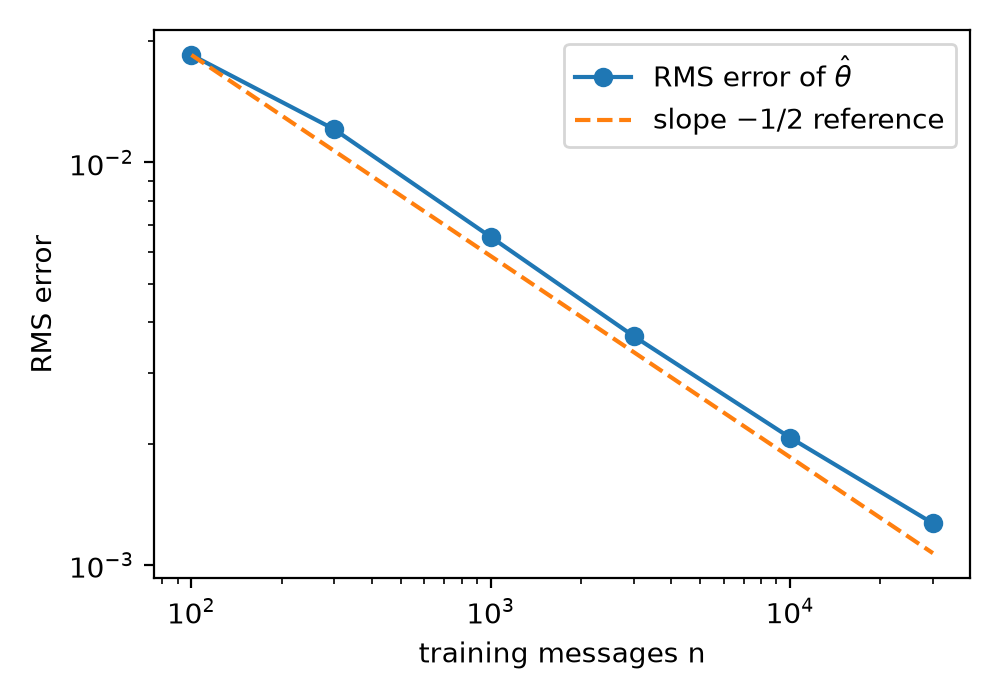
\includegraphics[width=0.47\textwidth]{sim_theta_error_vs_n.png}\hfill
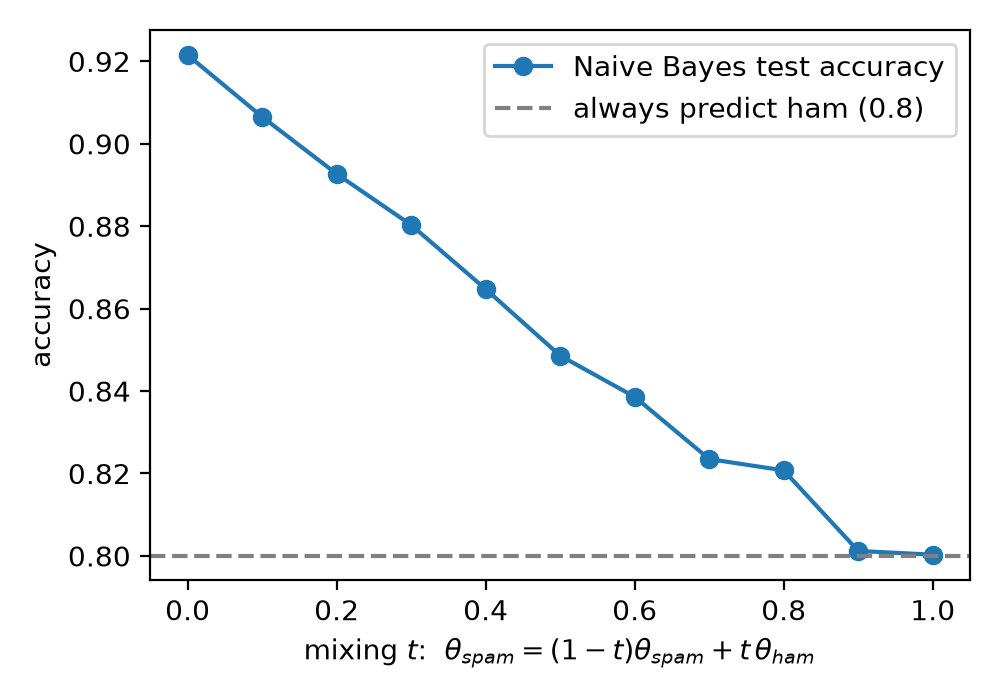
\includegraphics[width=0.47\textwidth]{sim_accuracy_vs_similarity.png}
\caption{Left: RMS error of $\hat\Theta$ falls like $n^{-1/2}$ (mean of 20 runs).
Right: accuracy falls as the spam distribution is mixed toward the ham distribution,
reaching the ``always ham'' baseline of 0.80 when they are equal.}
\label{fig:sim}
\end{figure}

\textbf{What each result confirms.}
\begin{itemize}[leftmargin=*]
\item \textbf{Q1 (Theorem~\ref{thm:posterior}):} with data that satisfy conditional independence,
the classifier built from the factorized posterior reaches 0.910 accuracy, close to the 0.918
obtained with the true parameters.
\item \textbf{Q2 (Theorem~\ref{thm:mle}):} the count ratio equals the code's MLE to machine
precision, the estimates are within 0.011 of the truth (Table~\ref{tab:sim}), and the error
shrinks like $n^{-1/2}$ (Figure~\ref{fig:sim}, left).
\item \textbf{Q3 (Prop.~\ref{prop:zero}, Theorem~\ref{thm:laplace}):} when spam can never emit
word $w_0$, a message containing $w_0$ gets spam log-score $-\infty$ without smoothing and a
finite score with $\alpha=1$; smoothed rows sum to exactly 1.
\item \textbf{Q4 (Theorem~\ref{thm:linear}):} the score difference equals $X\bw+b$ to
$10^{-15}$, and the argmax of the log-scores equals the argmax of the posteriors for all 400
test messages.
\item \textbf{Q5 (Prop.~\ref{prop:prec}, Theorem~\ref{thm:wilson}):} the classifier's true
precision and recall, measured on 200{,}000 fresh messages (0.848 and 0.762), lie inside our
intervals, and repeated test sets give 94.6\% coverage, close to the nominal 95\%.
\item \textbf{D1, D2:} the Dirichlet-mean formula is the same expression the code uses for
$\alpha=1$; posterior probabilities from log-sum-exp sum to 1.
\end{itemize}
\owner{Jeevan Mandala}{Anand Joel Battula}

%======================================================================
\clearpage
\appendix
\section{Hand-Worked Example}\label{app:hand}
\textbf{Data.} Vocabulary $\V=\{\text{free},\text{win},\text{call},\text{meet}\}$, $\Vs=4$, $\alpha=1$.
\begin{center}
\begin{tabular}{@{}llcccc@{}}
\toprule
Message & Class & free & win & call & meet\\
\midrule
$d_1$ ``free win free'' & spam & 2 & 1 & 0 & 0\\
$d_2$ ``win call'' & spam & 0 & 1 & 1 & 0\\
$d_3$ ``call meet'' & ham & 0 & 0 & 1 & 1\\
$d_4$ ``meet call meet'' & ham & 0 & 0 & 1 & 2\\
\bottomrule
\end{tabular}
\end{center}

\textbf{Step 1: counts} ($C=Y^\top X$). Spam: $(2,2,1,0)$, $N_1=5$. Ham: $(0,0,2,3)$, $N_0=5$.

\textbf{Step 2: priors.} $\hat\pi_1=\hat\pi_0=2/4=1/2$ (Theorem~\ref{thm:mle}).

\textbf{Step 3: smoothed probabilities} (Theorem~\ref{thm:laplace}), denominator $N_c+\Vs=9$:
\[
\tilde{\boldsymbol\theta}_{\text{spam}}=\Big(\tfrac39,\tfrac39,\tfrac29,\tfrac19\Big),\qquad
\tilde{\boldsymbol\theta}_{\text{ham}}=\Big(\tfrac19,\tfrac19,\tfrac39,\tfrac49\Big).
\]
Each row sums to $9/9=1$.

\textbf{Step 4: classify} $t_1=$ ``free meet'', $\bx=(1,0,0,1)$ (Theorem~\ref{thm:posterior}):
\[
\text{spam: }\tfrac12\cdot\tfrac39\cdot\tfrac19=\tfrac{3}{162},\qquad
\text{ham: }\tfrac12\cdot\tfrac19\cdot\tfrac49=\tfrac{4}{162},\qquad
P(\text{spam}\mid t_1)=\frac{3}{3+4}=\frac37\approx0.4286.
\]
Prediction: ham. For $t_2=$ ``free call'', $\bx=(1,0,1,0)$: spam $\tfrac12\cdot\tfrac39\cdot\tfrac29=\tfrac6{162}$,
ham $\tfrac12\cdot\tfrac19\cdot\tfrac39=\tfrac3{162}$, so $P(\text{spam}\mid t_2)=6/9=2/3$. Prediction: spam.

\textbf{Step 5: linear rule} (Theorem~\ref{thm:linear}).
$\bw=\log\tilde{\boldsymbol\theta}_{\text{spam}}-\log\tilde{\boldsymbol\theta}_{\text{ham}}
=(\log3,\ \log3,\ \log\tfrac23,\ \log\tfrac14)\approx(1.0986,\,1.0986,\,-0.4055,\,-1.3863)$, $b=\log\frac{1/2}{1/2}=0$.
For $t_1$: $\bw^\top\bx=\log3+\log\frac14=\log\frac34\approx-0.2877<0$ (ham), and
$e^{-0.2877}=3/4$ is the spam-to-ham odds, consistent with $3/7$. For $t_2$:
$\log3+\log\frac23=\log2\approx0.6931>0$ (spam).

\textbf{Step 6: without smoothing} ($\alpha=0$). $\hat\theta_{\text{meet}\mid\text{spam}}=0/5$ and
$\hat\theta_{\text{free}\mid\text{ham}}=0/5$, so both scores of $t_1$ are 0 and
$P(\text{spam}\mid t_1)=0/0$ is undefined (Proposition~\ref{prop:zero}).

\textbf{Code check.} \texttt{src/hand\_example.py} gives $\tilde\Theta$ with maximum difference
$1.4\times10^{-17}$ from the fractions above, posteriors $(0.428571,\,0.666667)$ with maximum
difference $1.1\times10^{-16}$ from $(3/7,\,2/3)$, the same $\bw$, and log-scores
$(-\infty,-\infty)$ for $t_1$ when $\alpha=0$.
\owner{Jeevan Mandala}{Anand Joel Battula}

\section{Reproducibility}
All code is in \texttt{src/} and uses only \texttt{numpy}, \texttt{pandas}, \texttt{matplotlib}
and \texttt{scipy.stats}. From the repository root, run
\begin{center}
\texttt{python src/hand\_example.py}\qquad
\texttt{python src/simulation.py}\qquad
\texttt{python src/load\_data.py}
\end{center}
See \texttt{README.md} for how to download the data.

\end{document}
